\documentclass[runningheads]{llncs}

\usepackage[utf8]{inputenc}
\usepackage{graphicx}
\usepackage{mathpazo}
\usepackage{todonotes}

% Todo commands

\newcommand{\todoin}[2][]{\todo[inline, color=blue!40, #1]{#2}}
\newcommand{\fixme}[2][]{\todo[color=yellow!40, #1]{#2}}
\newcommand{\fixmein}[2][]{\todo[inline, color=yellow!40, #1]{#2}}


% If you use the hyperref package, please uncomment the following line
% to display URLs in blue roman font according to Springer's eBook style:
% \renewcommand\UrlFont{\color{blue}\rmfamily}

\begin{document}

\title{Ant Colony Optimization algorithms \\
for the Permutation Flow Shop Problem with Weighted Tardiness}
\subtitle{}

\titlerunning{ACO algorithms for PFSP-WT}

\author{Hakim Boulahya \\
hboulahy@ulb.ac.be}

\authorrunning{H. Boulahya}

\institute{Université Libre de Bruxelles}

\maketitle

\begin{abstract}
In this article we present two Ant Colony Optimization algorithms for the
permutation flow shop problem with weighted tardiness.

\keywords{First keyword  \and Second keyword \and Another keyword.}
\end{abstract}

\section{Introduction}

\fixmein{Check FIXME in source code}

(see Fig.~\ref{fig1})

\begin{figure}
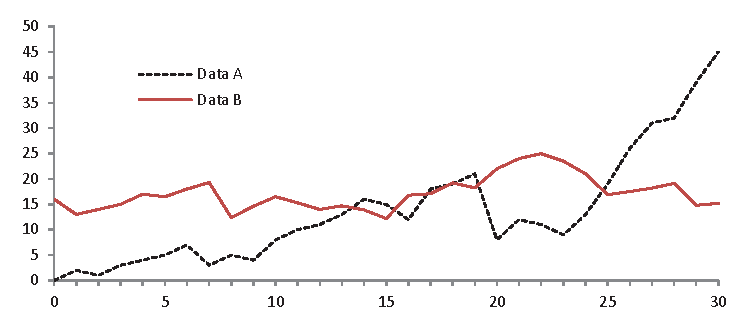
\includegraphics[width=\textwidth]{figures/fig1.eps}
\caption{A figure caption is always placed below the illustration.
Please note that short captions are centered, while long ones are
justified by the macro package automatically.} \label{fig1}
\end{figure}

\subsection{Problem description}

\section{Ant Colony Optimization algorithm for PFSP-WT}

\subsection{Ant Colony System}



\subsubsection{Solution representation} For the PFSP-WT problem, a solution is a permutation of jobs
that must be scheduled and executed.
The objective is to minimize the sum weighted tardiness
$\sum_{i=1}^{n}{w_i T_i}$ of a permutation of jobs.


\paragraph{Note:} when not specified $\tau_{ij}$ and $\eta_{ij}$ correspond to $\tau_{ij}(t)$ and $\eta_{ij}(t)$,
where $\tau_{ij}(t)$ is the pheromone trail of the job $i$ in position $j$ of the current schedule and.


\paragraph{Heuristic information}


\subsubsection{Schedule construction}
\fixmein{Schedule vs iteration vs try (chck acotsp v1.0.3) ?}

\paragraph{}


With probability $q_0$ ants will sechedule the job $i$ at position $j$ that maximize $(\tau_{ij})^\alpha (\eta_{ij})^\beta$, that is $\mathrm{argmax}_{unscheduled}(\tau_{ij})^\alpha (\eta_{ij})^\beta$

\paragraph{}


Ant explore with probabilibty $1 - q_0$ where the probability distribution to select an unscheduled job is:

\begin{equation}
p_{ij} = \frac{(\tau_{ij})^\alpha (\eta_{ij})^\beta}{\sum_{unscheduled}{(\tau_{ij})^\alpha (\eta_{ij})^\beta}}
\end{equation}

\subsubsection{Pheromone}


\subsubsection{Heuristic}

$\eta_{ij}$ is the heuristic information (when combined with $\tau_{ij}$
it is the desirabity of putting job $i$ in position $j$ \cite{den_besten_ant_2000}).

\todoin{Implement NEH heuristic}

\subsubsection{Global Pheromone Trail Update}

Same update from \cite{den_besten_ant_2000}.



\begin{equation}
\tau_{ij}(t+1) = (1 - \rho) \cdot \tau_{ij}(t) + \rho \cdot \Delta \tau_{ij}(t)
\end{equation}

where $\Delta \tau_{ij}(t)$ = $ 1 / T^{*}$ with $T^*$ the total weighted tardiness of the current solution.

\subsubsection{Local Pheromone Trail Update}

Same update from \cite{den_besten_ant_2000} and
extented definition from \cite{dorigo_ant_2004} for parameters $\tau_0$.

During schedule construction, each time an ant add a job $i$ in position $j$ the following update rule is applied:

\begin{equation}
\tau_{ij} = (1 - \xi) \cdot \tau_{ij} + \xi \cdot \tau_{0}
\end{equation}

Where $0 < \xi \le 1$ and $\tau_0$ is set as the initial value of the pheromone trails set to $\tau_0 = 1 / n \cdot T_{h}$ \cite{den_besten_ant_2000} where $n$ is the number of jobs and
$T_h$ the total weighted tardiness of the solution generated by the heuristic $h$.

\subsection{$\mathcal{MAX – MIN}$ Ant System}

Inspired from \cite{stutzle_ant_1997}.

\subsubsection{Solution representation} Same as ACS

\subsubsection{Schedule construction} Same as ACS

\subsection{Heuristic} Same as ACS

\subsubsection{Global Pheromone Trail Update}

\begin{equation}
\tau_{ij}(t+1) = (1 - \rho) \cdot \tau_{ij}(t) + \Delta \tau_{ij}(t)
\end{equation}

\fixmein{Why there is not $\rho$ multiplied with $\Delta$ Book + Thomas does not use $\rho$
and THomas uses only $1 - \rho$ ?}

\subsubsection{Pheromone Trails Limits}

$\tau_{max}$ is set set to $1 / \rho T^*$ and upated at each iteration, each time a new
best-so-far is found.
$\tau_{min} = \tau_{max} / a$ where a is set to $5$ \cite{stutzle_ant_1997}.

\subsubsection{Pheromone Trails Initialization and Reinitialization}

\todoin{See how to detect stagnation of the trails and what formula to use for reinit.}








\todoin{Below are just draft notes}



Extension from \cite{dorigo_ant_2004}.

Inspired from \cite{den_besten_ant_2000}.


\section{Experimental results}

\subsection{Tuning}

\todoin{Include table with param, type, range and why}

\todoin{For parameters range see ACOTSP irace example}

\subsection{}


\bibliographystyle{splncs04}
\bibliography{SWARM}

\end{document}
